\section{実験1-2}
\subsection{実験の目的,概要}
この実験では,実験1-1で正しく動作しなかったプロセッサに,新たに命令実装を追加し,同じプログラムを実行,結果を確認する。
また,実験1-1で行った予想と比較する。

これによって,プロセッサに命令を追加する方法,配線図を実装に反映させる方法を確認することを目的とする。

\subsection{実験方法}
\subsubsection{addiu命令の追加設計}
以下の点について,main\_ctrl.vを編集した。
\begin{lstlisting}[caption={addiu命令の追加設計},label={addiu命令の追加設計}]
// 命令コードの定義を追加
`define ADDIU 6'b001001

// 分岐判定のコントロール信号を追加
`ADDIU: is_branch_ctrl_tmp = 3'b110;

// オペランドに即値,レジスタのどちらをとるのかの制御信号の追加
`ADDIU: alu_b_sel1_s_tmp = 1'b1;

// 即値の符号拡張が行われるかどうかのフラグを追加
(op_code == `ADDIU)

// ALUがどの演算を行うかの制御信号の追加
`ADDIU: alu_op_tmp = 3'b000;

// レジスタへの書き込み制御信号を追加
`ADDIU:  reg_write_enable_tmp = 1'b1;

// ALUの演算結果とRAMの内容のセレクト信号を追加
`ADDIU:  alu_ram_sel_s_tmp = 1'b0;

// RtとRdのセレクト信号の追加
`ADDIU:  reg_widx_sel1_s_tmp = 1'b0;

// レジスタに書き込む,ALUの出力orRAMのデータと,PCの値のセレクタ信号の追加
`ADDIU:  link_tmp = 1'b0;

\end{lstlisting}

\subsubsection{sw命令の追加設計}
以下の点について,main\_ctrl.vを編集した。
\begin{lstlisting}[caption={sw命令の追加設計},label={sw命令の追加設計}]
// 命令コードの定義を追加
`define SW 6'b101011 // store word (I 形式)

// RAMへの書き込みを制御する信号を追加
assign ram_write_enable = (op_code == `SW) ? 1'b1 : 1'b0;

// 分岐判定のコントロール信号を追加
`SW: is_branch_ctrl_tmp = 3'b110; // do nothing

// 即値とRtレジスタのセレクト信号を追加
`SW: alu_b_sel1_s_tmp = 1'b1;

// 即値の符号拡張が行われるかどうかのフラグを追加
|| (op_code == `SW)

// ALUがどの演算を行うかの制御信号の追加
`SW: alu_op_tmp = 3'b000;

// レジスタへの書き込み制御信号の追加
`SW: reg_write_enable_tmp = 1'b0;

\end{lstlisting}

\subsubsection{論理合成,FPGAでの回路実現}
以下のように,コンパイルを行ない,dmesgで接続を確認した。
その後FPGAにダウンロードして,FPGAでの動作を確認した。

\begin{lstlisting}[caption={コンパイル,ダウンロード},label={コンパイル,ダウンロード1-2}]
  $ quartus_sh --flow compile MIPS_Default
  $ quartus_pgm MIPS_Default.cdf 
\end{lstlisting}

実行時には,1-1で予想した以下の点について確認する。
\begin{itemize}
  \item PC=0x0040 002cの命令を実行したときの,REG[2]の値
  \item PC=0x0040 0030の命令を実行したときの,RAMの768番地の値
  \item PC=0x0040 0034の命令を実行したときの,REG[3]の値
  \item PC=0x0040 003cの命令を実行したとき,RAMの何番地の値がどう変化するか
  \item PC=0x0040 0048の命令を実行したとき,RAMの何番地の値がどう変化するか
\end{itemize}

\subsubsection{機能レベルシュミレーション}
以下のように,cou.vを編集した。
\begin{itemize}
  \item cpu.v の 70 行目周辺,動作実験用の include 文をコメントアウトした。
  \item cpu.v の 65 行目周辺,機能レベルシミュレーション用 include を有効にした。
  \item cpu.v の 320 行目周辺,動作実験用の ROM の実体化を数行コメントアウトした。
  \item cpu.v の 315 行目周辺,機能レベルシミュレーション用の ROM の実体化を有効にした。
  \item cpu.v の 340 行目周辺,動作実験用の RAM の実体化を数行コメントアウトした。
  \item cpu.v の 335 行目周辺,機能レベルシミュレーション用の RAM の実体化を有効にした。
\end{itemize}

以下の操作によって,シュミレーション用ROMファイルをMIPS以下にコピーし,Modelsimを起動して機能レベルシュミレーションを行なった。

\begin{lstlisting}[caption={機能レベルシュミレーション},label={機能レベルシュミレーション1-2}]
  $ cp rom8x1024_sim.v /mips_de10-lite/MIPS
  $ cd /mips_de10-lite/MIPS
  $ vsim test_cpu.v
\end{lstlisting}

シュミレーション終了後,cpu.vで変更した部分はもとに戻した。

\subsection{実験結果}
\subsubsection{論理合成,FPGAでの回路実現}
ダウンロードして実行すると,画面上に'B'という文字が表示された。

実験1-1で行った予想との比較は,以下のように予想通りの結果になった。
\begin{itemize}
  \item PC=0x0040 002cの命令を実行したときの,REG[2]の値
  \begin{itemize}
    \item 768が書き込まれた
  \end{itemize}
  \item PC=0x0040 0030の命令を実行したときの,RAMの768番地の値
  \begin{itemize}
    \item 0が書き込まれた
  \end{itemize}
  \item PC=0x0040 0034の命令を実行したときの,REG[3]の値
  \begin{itemize}
    \item 772が書き込まれた
  \end{itemize}
  \item PC=0x0040 003cの命令を実行したとき,RAMの何番地の値がどう変化するか
  \begin{itemize}
    \item RAM[772]に2が書き込まれた
  \end{itemize}
  \item PC=0x0040 0048の命令を実行したとき,RAMの何番地の値がどう変化するか
  \begin{itemize}
    \item RAM[768]に1が書き込まれて,その前にはPC=0x0030でRAM[REG[2]→768]に0が書き込まれていた
  \end{itemize}
\end{itemize}

\subsection{機能レベルシュミレーション}
機能レベルシュミレーションの結果、波形は以下のようになった。
\begin{figure}[H]
  \centering
  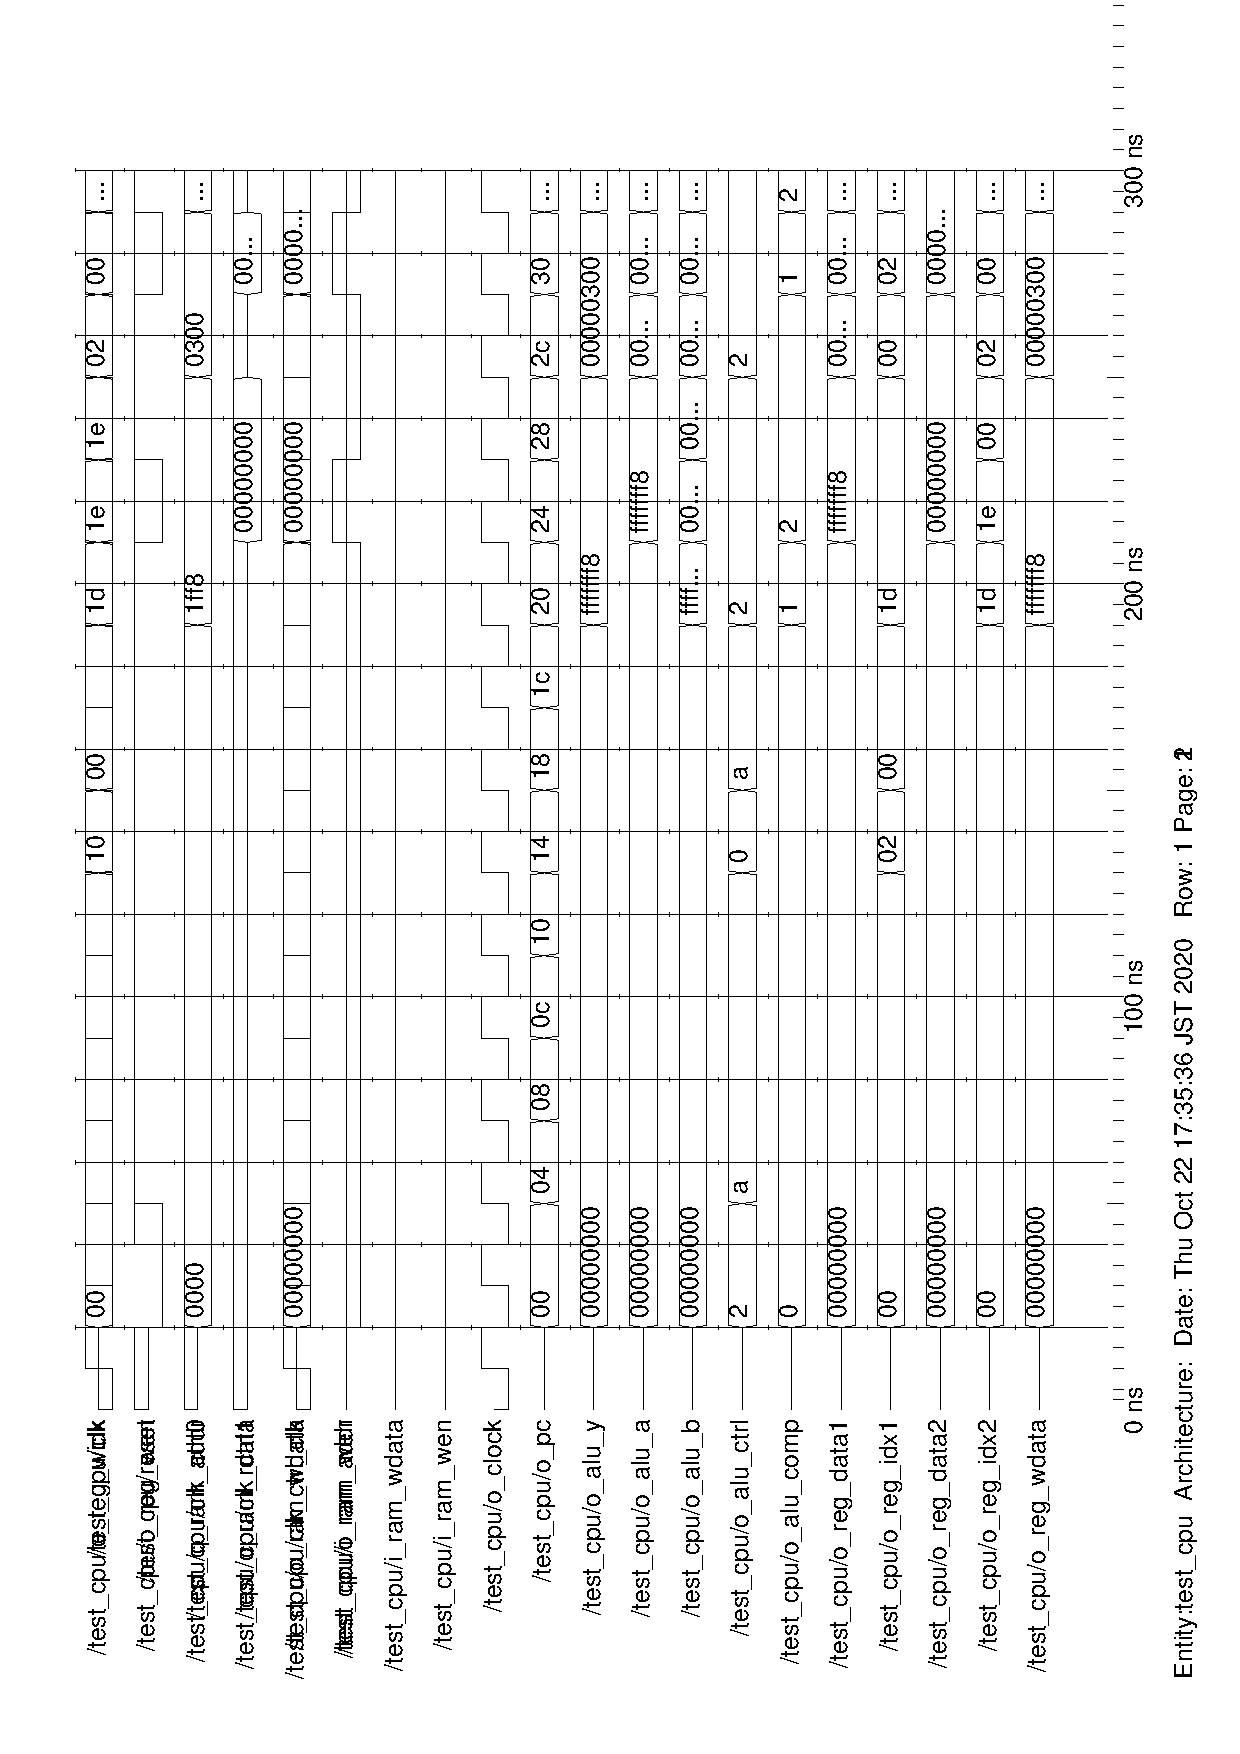
\includegraphics[width=\linewidth]{./src/01/testCPUwave.png}
  \caption{プロセッサの波形}
\end{figure}

\subsection{考察}
